%%%%%%%%%%%%%%%%%%%%%%%%%%%%%%%%%%%%%%%%%%%%%%%%%%%%%%%%%%%%
% % Title and the authors % %
%%%%%%%%%%%%%%%%%%%%%%%%%%%%%%%%%%%%%%%%%%%%%%%%%%%%%%%%%%%%
\title{Lagrange Multipliers}
\author{ Gabriela Georgieva \\ Angelina Kuznetsova \\ Fedor Shafranov} \date{\today } 
\documentclass[]{article}

\usepackage{graphicx}
\usepackage[utf8]{inputenc}
\usepackage{setspace}
\usepackage{amsthm}
\usepackage{amssymb}
\usepackage{amsmath}
\usepackage{hyperref}
\usepackage{tikz}
\usetikzlibrary{matrix}

\newtheorem{theorem}{Theorem}
\newtheorem{lemma}{Lemma}
\newtheorem{example}{Example}
\newtheorem{problem}{Problem}
\newtheorem{proposition}{Proposition}
\newtheorem{scolium}{Scolium} 
\newtheorem{definition}{Definition}

\newcommand{\R}{\mathbb{R}}
\newcommand{\Z}{\mathbb{Z}}
\newcommand{\X}{\mathbb{X}}
\newcommand{\imply}{\Rightarrow}

\graphicspath{{images/}} 

\begin{document} 
\maketitle
\begin{abstract}
    Oftentimes one wants to find a minima or maxima of a (differentiable) function subject to one or more constraints. An elegant way to find an extremum is by using the so-called Lagrange Multipliers. Lagrange Multipliers are handy when solving optimization problems in Economics, Business, Computer Science, etc. 
\end{abstract}
\begin{figure}[h]
    \centering
    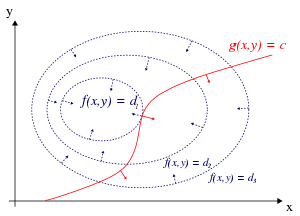
\includegraphics[width=0.50\textwidth]{abstract_img.png}
\end{figure}


\newpage
\tableofcontents
\newpage

\section{Lagrange Multipliers}
%%%%%%%%%%%%%%%%%%%%%%%%%%%%%%%%%%%%%%%%%%%%%%%%%%%%%%%%%%%%%%%%%%%%%%%%%%%%%%%%%%%%%
\subsection{Introduction}

\begin{theorem}(Implicit Function Theorem) \\
    Suppose that $F:\mathbb{R}^{n+1}\to \mathbb{R}$ is $C^{1}$. We will denote points in $\mathbb{R}^{n+1}$ 
    by ($\pmb{x}$,$z$), where $\pmb{x}\in \mathbb{R}^n$ and $z\in \mathbb{R}$. Assume \\
    $$
        F(\pmb{x}_{0},z_{0})=c \hspace{30pt} and \hspace{30pt} \nabla F(\pmb{x}_{0},z_{0})\neq \pmb{0}
    $$
    Then there is a ball $U$ that contains $\pmb{x}_{0}$ and a neighborhood $V$ of $z_{0}$ in $\mathbb{R}$ such that there is a function $z=g(\pmb{x})$ defined for $\pmb{x}$ in $U$ and $z$ in $V$ that satisfies
    $$
        F(\pmb{x},g(\pmb{x}))=c
    $$
    
\end{theorem}

\begin{theorem}(Method of Lagrange Multipliers) \\
    Suppose that $f:\mathbb{R}^{n}\to \mathbb{R}$ and $g:U\subset\mathbb{R}^{n}\to \mathbb{R}$ are $C^{1}$. Let $\pmb{x}_{0}\in U$ and $g(\pmb{x}_{0})=c$, and let $S$ be the level set for $g$ with value $c$ (i.e these are the set of points $\pmb{x}\in \mathbb{R}^{n}$ that satisfy $g(\pmb{x})=c$).
    Assume $\nabla g(\pmb{x}_{0})\neq \pmb{0}$. \\
    If $(\pmb{x}_{0})$ is a local extremum, then there exists $\lambda$ such that
    $$
        \nabla f(\pmb{x}_{0}) = \lambda \nabla g(\pmb{x}_{0})
    $$
\end{theorem}

\subsection{Single Constraint}
%%%%%%%%%%%%%%%%%%%%%%%%%%%%%%%%%%%%%%%%%%%%%%%%%%%%%%%%%%%%%%%%%%%%%%%%%%%%%%%%%%%%%

\subsection{Multiple Constraints}
%%%%%%%%%%%%%%%%%%%%%%%%%%%%%%%%%%%%%%%%%%%%%%%%%%%%%%%%%%%%%%%%%%%%%%%%%%%%%%%%%%%%%

\subsection{Second Derivative Test}
%%%%%%%%%%%%%%%%%%%%%%%%%%%%%%%%%%%%%%%%%%%%%%%%%%%%%%%%%%%%%%%%%%%%%%%%%%%%%%%%%%%%%

\subsection{Lagrangian}
%%%%%%%%%%%%%%%%%%%%%%%%%%%%%%%%%%%%%%%%%%%%%%%%%%%%%%%%%%%%%%%%%%%%%%%%%%%%%%%%%%%%%

\section{Applications}
%%%%%%%%%%%%%%%%%%%%%%%%%%%%%%%%%%%%%%%%%%%%%%%%%%%%%%%%%%%%%%%%%%%%%%%%%%%%%%%%%%%%%

\end{document}
